\documentclass[xetex,aspectratio=43]{beamer}

\usepackage{res/lections}

\preamble

\title[Докомпьютерные, Эйкен, фон Нейман]{Докомпьютерные вычислители, архитектуры~Эйкена~и~фон~Неймана}

\begin{document}

\titleslide

\tocslide

\section{Краткая история цифровой
		вычислительной техники}

\subsection{История вычислительной техники до XX века}

\begin{frame}{История вычислительной техники до XIX века}
	\begin{block}{XVII век}
		\begin{itemize}
			\item
			\href{https://en.wikipedia.org/wiki/Pascal\%27s_calculator\#Addition}{Сумматор
				Паскаля~\extlink} --- складывал; вычитал при помощи дополнительного кода
			\item
			\href{https://en.wikipedia.org/wiki/Stepped_reckoner\#Operation}{Арифмометр
				Лейбница~\extlink} --- складывал, вычитал, сдвигал; при помощи этого позволял
			умножать и делить
		\end{itemize}
	\end{block}

	\pause

	\begin{block}{XIX век}
		\begin{columns}
		\begin{column}{0.7\textwidth}
			\begin{itemize}
				\item
				\href{https://en.wikipedia.org/wiki/Charles_Babbage\#Computing_pioneer}{Машины
					Беббиджа~\extlink}
	
				\item
				\href{https://en.wikipedia.org/wiki/Odhner_Arithmometer}{Арифмометр
					Однера~\extlink} --- изобретён в Санкт-Петербурге шведом Однером. Умеет то же,
				что и арифмометр Лейбница, но компактный и дешёвый
			\end{itemize}
		\end{column}
		\begin{column}{0.3\textwidth}
			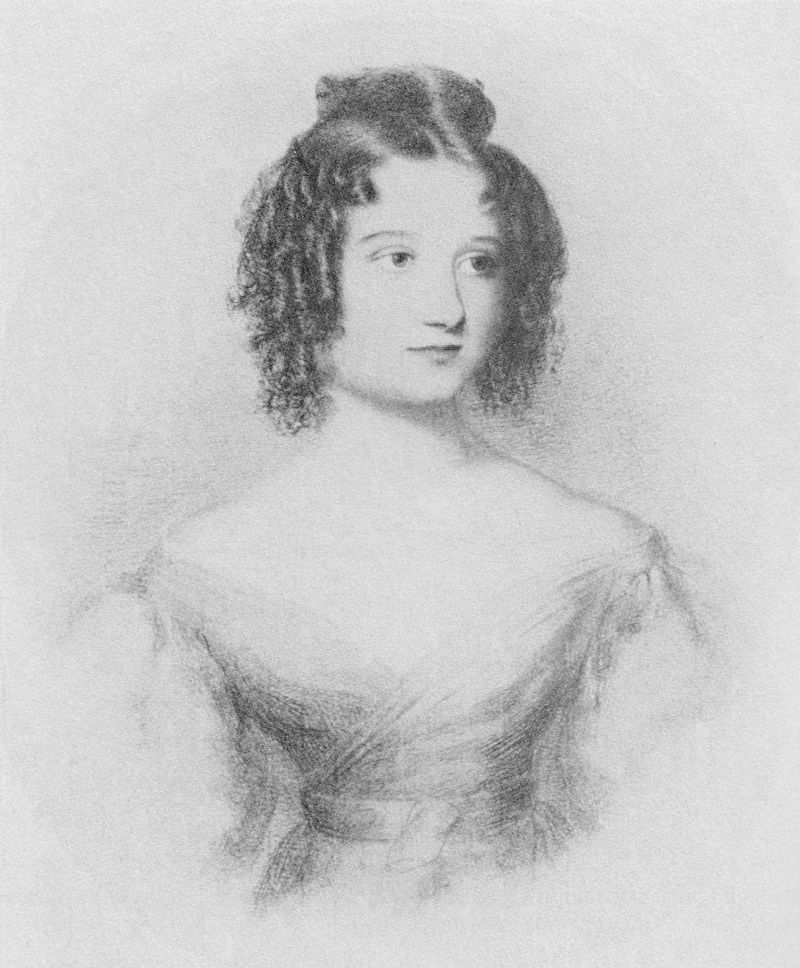
\includegraphics[width=\textwidth]{img/02.Ada_Byron_aged_seventeen_1832.jpg}
		\end{column}
		\end{columns}
	\end{block}
\end{frame}

\begin{frame}{Вычислительная техника конца XIX -- начала XX в.}
	\href{https://en.wikipedia.org/wiki/Tabulating_machine}{Табуляторы~\extlink}
	
	\begin{itemize}
		\item
		Hollerith
		\item
		IBM
		
		\begin{itemize}
			\item
			\href{https://en.wikipedia.org/wiki/IBM_407}{IВM 407~\extlink} выпускался до
			1976 г.!
		\end{itemize}
	\end{itemize}
	
	Табуляторы могли обрабатывать (сортировать, фильтровать) массивы данных,
	но они не программировались.
\end{frame}

\section{XX век, программируемые вычислительные машины}

\subsection{Специализированные вычислительные устройства}

\begin{frame}{Colossus}
	
		1940-е \href{https://en.wikipedia.org/wiki/Colossus_computer}{Colossus~\extlink}
		--- машина для взлома шифра Лоренца (продолжение Энигмы).
		
		Ламповая ЭВМ, по производительности универсальные микропроцессоры
		обогнали её только в конце 1980-х. Рассекречена в 2000 г.

\end{frame}

\subsection{Универсальные вычислительные устройства}

\begin{frame}{1930-е -- 1940-е, <<Гарвардская>> (Эйкена) архитектура}
		\begin{itemize}
			\item
			\href{https://en.wikipedia.org/wiki/Z1_(computer)}{Z1~\extlink}
		\pause
			\item
			\href{https://en.wikipedia.org/wiki/Harvard_Mark_I}{Harvard Mark I~\extlink}.
			Говард Эйкен. Фактически, вычислитель, управляемый перфолентой.
		\end{itemize}
				
		\begin{figure}
			\includesvg[height=0.5\textheight]{img/02.Harvard.svg}
		\end{figure}
		
		\pause
		А управляемый ли?.. Переходов нет, циклы --- при помощи склеивания перфоленты в кольцо.
\end{frame}

\begin{frame}{Немного терминов}
	\begin{itemize}
		\item
		\defn{Центральный процессор}{устройство, выполняющее программу}
		\item
		\defn{Машинный код}{язык, задающий числовое представление
		инструкций программы}
		\item
		\defn{Оперативная память (ОЗУ, RAM)}{память, хранящая данные
		и/или машинный код}
	\end{itemize}
\end{frame}

\begin{frame}{1940-е -- \ldots <<Принстонская>> (фон Неймана) архитектура}
	\begin{figure}
		\includesvg[height=0.5\textheight]{img/02.Von_Neumann_Architecture.svg}
	\end{figure}
	
	\pause
	
	\begin{enumerate}
		\item
		Программное управление работой ЭВМ
		\item
		\em{Принцип хранимой программы}
		\item
		Использование двоичной системы исчисления
		\item
		Иерархичность запоминающих устройств
		\item
		Использование условных переходов
	\end{enumerate}
\end{frame}

\begin{frame}{Системная шина фон Неймановских машин}
		\begin{figure}
			\includesvg[height=0.5\textheight]{img/02.Von_Neumann_System_Bus.svg}			
		\end{figure}
		
		\pause
		
		Системная шина --- узкое место с точки зрения производительности. В
		процессорах современных ЭВМ используются элементы гарвардской
		архитектуры --- отдельные виды кэш-памяти для данных и машинного кода.
\end{frame}

\begin{frame}{Современные гарвардские вычислители}
	\begin{itemize}
		\item
		Встраиваемые контроллеры (лифты, стиральные машины, коробки скоростей)
		\item
		Специализированные устройства
	\end{itemize}
		
		Т.е. устройства, которые не надо часто перепрограммировать. Для них нет
		смысла рассматривать программу, как данные. Например, у некоторых
		микроконтроллеров производства компании Microchip память для кода
		делится на 12-битные ячейки.

	\pause
	
	\begin{itemize}
		\item Контроллеры (например, Serial ATA) в <<традиционных>> компьютерах
		\item Шейдеры в графических адаптерах
	\end{itemize}

	Т.е. устройства, от которых требуется высокая производительность на единицу цены,
	но не требуется возможности <<самостоятельно>> программироваться.
		
\end{frame}

\section{Поколения ЭВМ}

\begin{frame}{I поколение: 1940-е, в основном физические вычисления}
	
	\begin{block}{Свойства}
		\begin{itemize}
			\item
			Процессор на ламповых диодах и триодах
			\item
			Память на электромагнитных реле
		\end{itemize}
		
		Процессор на реле --- слишком медленно, частота срабатывания реле ---
		несколько Гц. \href{https://youtu.be/5hhbGBlP3_4}{Современный пример~\extlink}
	\end{block}
	
	\begin{block}{Примеры}
		ENIAC, EDVAC, Z4, МЭСМ, «Урал», «Стрела»
	\end{block}
	
	\begin{block}{Масштабы}
		\begin{itemize}
			\item
			ENIAC (1947 г.) --- 30 тонн, 200 кВт
			\item
			доступны крупным научно-исследовательским институтам, военным и
			государственным учреждениям
		\end{itemize}
	\end{block}
\end{frame}

\begin{frame}{II поколение: 1950-е -- 1960-е, в основном физические и экономические вычисления}

	\begin{block}{Свойства}
		\begin{itemize}
			\item
			Процессор на транзисторах
			\item
			Память на транзисторах или
			\href{https://en.wikipedia.org/wiki/Magnetic-core_memory}{материалах с
				магнитной памятью~\extlink}
		\end{itemize}
	\end{block}
	
	\begin{block}{Примеры}
		IBM 7094, CDC 1604, CDC 3600, БЭСМ-6
	\end{block}
	
	\begin{block}{Масштабы}
		\begin{itemize}
			\item
			Единицы тонн, единицы и десятки кВт
			\item
			Доступны университетам, крупным промышленным предприятиям (банки,
			заводы и т.д.), государственным учреждениям
		\end{itemize}
	\end{block}
\end{frame}

\begin{frame}{III поколение: 1960-е -- 1970-е, вычисления, «офисная» работа}
	
	
	\begin{block}{Свойства}
		\begin{itemize}
			\item
			Использование интегральных схем
		\end{itemize}
		
		\textbf{Интегральная схема} --- неразборная электронная схема на
		полупроводниковой подложке.
		
		Технология изготовления (упрощённо) --- фотолитография
		
		Степень интеграции и количество элементов в кристалле:
		
		\begin{itemize}
			\tightlist
			\item
			малая интегральная схема (МИС) --- \(\le 10^2\)
			\item
			средняя интегральная схема (СИС) --- \(\le 10^3\)
			\item
			большая интегральная схема (БИС) --- \(\le 10^4\)
			\item
			сверхбольшая интегральная схема (СБИС) --- \(> 10^4\)
		\end{itemize}
	\end{block}
	
	\begin{columns}
		\begin{column}{0.2\textwidth}
			\begin{block}{Примеры}
				\vspace{5mm}
				IBM-360, ЕС ЭВМ
				\vspace{6mm}
			\end{block}
		\end{column}
		\begin{column}{0.02\textwidth}\end{column}
		\begin{column}{0.75\textwidth}	
			\begin{block}{Масштабы}
				\begin{itemize}
					\item
					Десятки и сотни кг, сотни Вт -- десятки кВт
					\item
					Доступны организациям, предприятиям, крупным подразделениям
				\end{itemize}
			\end{block}
		\end{column}
	\end{columns}

\end{frame}

\begin{frame}{IV поколение: 1970-е -- 1980-е -- \ldots, вычисления, «офисная» работа, развлечения}

	\begin{block}{Свойства}
		\textbf{Микропроцессор} --- процессор, реализованный в виде одной
		интегральной схемы
		
		\emph{Важно}: переход количества в качество. Цена ЭВМ была принципиально
		снижена и достигла уровня цены автомобиля, а позже --- обычной бытовой
		техники.
	\end{block}
	
	\begin{block}{Примеры}
		Apple (разные), IBM PC, Commodore, ZX Spectrum
	\end{block}
	
	\begin{block}{Масштабы}
		\begin{itemize}
			\item
			Единицы г -- единицы кг, единицы -- сотни Вт
			\item
			Доступны частным лицам
		\end{itemize}
	\end{block}
\end{frame}

\section{Закон Мура}

\begin{frame}{Закон Мура}
	Г. Мур, Intel 1965, эмпирическая закономерность
	
	\defn{Закон Мура}{
		количество полупроводниковых элементов в
		интегральных схемах каждые два года удваивается, т.е. \href{https://en.wikipedia.org/wiki/Moore\%27s_law}{растёт экспоненциально~\extlink}
	}
	
	\pause
	
	Увеличение схем --- не самоцель, оно даёт увеличение производительности.
	Но в последние годы пределы, установленные физическими законами, всё
	ближе. Сейчас закон Мура выполняется уже за счёт распараллеливания.
\end{frame}

\section{Отечественные ЭВМ}

\begin{frame}{Отечественные ЭВМ}
	\begin{itemize}
		\item
		1940-е -- 1950-е --- МЭСМ (I пок), 1960-е --- БЭСМ (II пок) --- С.А.
		Лебедев
		\item
		1950-е -- 1970-е --- Сетунь (троичная) --- Н.П. Бруснецов
		\item
		1960-е -- 1980-е -- копирование ЭВМ III и IV поколений (увы)
		\item
		1980-е --- оригинальные стековые архитектура Самсон и Кронос. В 1990-е
		годы Самсон был базовой ЭВМ ракетных войск стратегического назначения
		России.
		\item
		Сейчас --- процессоры двойного назначения Эльбрус (оригинальные
		разработки, отставание по производительности от лидеров на 5--10 лет,
		по цене выше), Байкал (семейство MIPS + свои доделки), разработки на
		основе архитектуры RISC-V
	\end{itemize}
\end{frame}

\begin{frame}{Упражнения и вопросы}
	\begin{block}{Упражнения}
		Найдите информацию об различных исторически значимых ЭВМ, сделайте обзор
		одной-двух понравившихся вам
	\end{block}
	
	\begin{block}{Вопросы}
		\begin{itemize}
			\tightlist
			\item
			Перечислите основные принципы архитектуры фон Неймана.
			\item
			Расскажите о схеме типовой ЭВМ, созданной на основе архитектуры фон
			Неймана.
			\item
			Назовите узкое место архитектуры фон Неймана.
			\item
			Чем архитектура фон Неймана отличается от гарвардской?
			\item
			Приведите примеры современных «гарвардских» устройств.
			\item
			Назначение и спектр задач ЭВМ I поколения
			\item
			Появление каких технологий привело к созданию ЭВМ II поколения?
			\item
			Какие технологии легли в основу ЭВМ III поколения?
			\item
			Назовите ключевую особенность ЭВМ IV поколения?
			\item
			Сформулируйте закон Мура
			\item
			За счет чего реализуется закон Мура в настоящее время?
		\end{itemize}
	\end{block}
\end{frame}

\postamble

\end{document}